% ASTRO -- NASA Space Apps Challenge presentation
% Compile from this directory with:
% tectonic --keep-logs ASTRO_presentation.tex
\documentclass[aspectratio=169,11pt]{beamer}

\usepackage[utf8]{inputenc}
\usepackage[T1]{fontenc}
\usepackage{lmodern}
\usepackage{graphicx}
\usepackage{xcolor}
\usepackage{booktabs}
\usepackage{tikz}
\usetikzlibrary{positioning}

\definecolor{astroblue}{HTML}{0B1026}
\definecolor{astroyellow}{HTML}{F0E442}
\definecolor{astroteal}{HTML}{009E73}
\definecolor{astrogray}{HTML}{667085}

\usetheme{default}
\setbeamertemplate{navigation symbols}{}
\setbeamertemplate{footline}{%
  \hbox{%
    \begin{beamercolorbox}[wd=.82\paperwidth,ht=2.5ex,dp=1ex,leftskip=1em]{author in head/foot}%
      \color{astrogray}\scriptsize ASTRO -- Your Little Big Commander
    \end{beamercolorbox}%
    \begin{beamercolorbox}[wd=.18\paperwidth,ht=2.5ex,dp=1ex,center]{date in head/foot}%
      \color{astrogray}\scriptsize\insertframenumber/\inserttotalframenumber
    \end{beamercolorbox}%
  }%
}
\setbeamercolor{normal text}{fg=astroblue,bg=white}
\setbeamercolor{frametitle}{fg=astroblue}
\setbeamercolor{structure}{fg=astroteal}
\setbeamercolor{alerted text}{fg=astroyellow!80!black}
\setbeamerfont{frametitle}{series=\bfseries,size=\Large}
\setbeamertemplate{itemize item}{\color{astroteal}\small\raisebox{0.15ex}{\(\blacktriangleright\)}}
\setbeamertemplate{itemize subitem}{\color{astroteal}\scriptsize\(\blacktriangleright\)}

\newcommand{\image}[2]{%
  \IfFileExists{../assets/figures/#1}{%
    \includegraphics[width=#2,height=.68\textheight,keepaspectratio]{../assets/figures/#1}%
  }{%
    \fbox{\parbox[c][.32\textheight][c]{.8\linewidth}{\centering\color{astrogray}Add \texttt{assets/figures/#1}}}%
  }%
}

\title{\textcolor{astroblue}{ASTRO}}
\subtitle{\textcolor{astroteal}{Your Little Big Commander}}
\author{Guardians of the Software Space Hawks}
\institute{NASA Space Apps Challenge 2026\\Build a Junior Astronaut Mission Trainer}
\date{}

\begin{document}

\begin{frame}
  \titlepage
  \vfill
  \begin{center}
    \small
    \href{https://astro.edu.us}{\textcolor{astroteal}{astro.edu.us}}
    \quad\textbullet\quad
    \href{https://github.com/ibanezbot-dev/NSAC-ASTRO}{\textcolor{astroteal}{GitHub}}
  \end{center}
\end{frame}

\begin{frame}{The challenge}
  \begin{columns}[T,onlytextwidth]
    \column{.55\textwidth}
      \textbf{Build a Junior Astronaut Mission Trainer}

      \medskip
      NASA Space Apps asks teams to transform the realities of operating a
      lunar or Martian outpost into an interactive mission experience.

      \medskip
      ASTRO responds with a playable system where:
      \begin{itemize}
        \item life support, radiation, energy, food, and science are connected;
        \item every decision creates a trade-off;
        \item consequences are visible, explainable, and replayable.
      \end{itemize}
    \column{.42\textwidth}
      \begin{center}
        \image{start-screen.jpeg}{\linewidth}
        \scriptsize A lunar base made understandable at a glance.
      \end{center}
  \end{columns}
\end{frame}

\begin{frame}{A mission built around decisions}
  \begin{columns}[T,onlytextwidth]
    \column{.52\textwidth}
      The player commands a four-person crew across four simulated lunar days.

      \medskip
      \begin{enumerate}
        \item Understand the situation.
        \item Choose how to spend limited resources.
        \item Predict what will happen.
        \item See the result and its cause.
        \item Replay with a new strategy.
      \end{enumerate}

      \medskip
      Players may send astronauts on a spacewalk, shelter them behind water
      shielding, invest energy in the greenhouse, use medical countermeasures,
      or save power for a later emergency.
    \column{.45\textwidth}
      \begin{center}
        \image{day1-gameplay.jpeg}{\linewidth}
        \scriptsize Prediction, action, feedback, and discovery.
      \end{center}
  \end{columns}
\end{frame}

\begin{frame}{Real NASA context, instant simulation}
  \begin{columns}[T,onlytextwidth]
    \column{.48\textwidth}
      \textbf{NASA data}
      \begin{itemize}
        \item DONKI space-weather events.
        \item OSDR space-biology context.
        \item NASA life-support and human-system references.
      \end{itemize}

      \medskip
      \textbf{Embedded intelligence}
      \begin{itemize}
        \item 6,000 NASA-anchored scenarios.
        \item Random Forest with 30 decision trees per output.
        \item JavaScript export for fast, offline browser inference.
      \end{itemize}
    \column{.48\textwidth}
      \begin{center}
        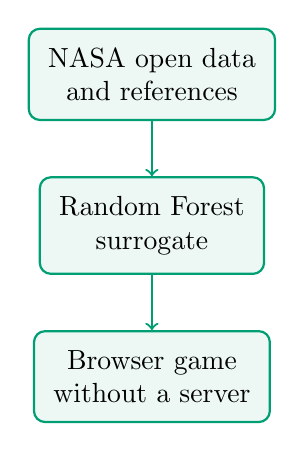
\begin{tikzpicture}[node distance=7mm, every node/.style={align=center, rounded corners, draw=astroteal, thick, fill=astroteal!7, inner sep=7pt}]
          \node (data) {NASA open data\\and references};
          \node (model) [below=of data] {Random Forest\\surrogate};
          \node (game) [below=of model] {Browser game\\without a server};
          \draw[->, thick, astroteal] (data) -- (model);
          \draw[->, thick, astroteal] (model) -- (game);
        \end{tikzpicture}

        \medskip
        \small
        The model translates storm intensity, shielding, activity,
        countermeasures, and greenhouse energy into cellular damage,
        crew efficiency, and crop health.
      \end{center}
  \end{columns}
\end{frame}

\begin{frame}{Designed for young explorers}
  \begin{columns}[T,onlytextwidth]
    \column{.52\textwidth}
      ASTRO makes complex systems concrete without turning the experience into
      a quiz.

      \medskip
      \begin{itemize}
        \item Two age modes for learners aged 7--12.
        \item Voice narration and short explanations.
        \item Glossary and guided tutorial.
        \item Keyboard navigation and reduced-motion support.
        \item Safe-to-fail missions that encourage curiosity and replay.
      \end{itemize}
    \column{.43\textwidth}
      \begin{center}
        \image{end-screen.jpeg}{\linewidth}
        \scriptsize A formative mission summary, not a grade.
      \end{center}
  \end{columns}
\end{frame}

\begin{frame}{Why ASTRO matters}
  \begin{center}
    \vspace{.15cm}
    {\Large\bfseries From space radiation to systems thinking}

    \vspace{.45cm}
    \begin{columns}[T,onlytextwidth]
      \column{.31\textwidth}
        \centering
        {\color{astroteal}\Large\bfseries Curiosity}

        \smallskip
        Children want to know what will happen if they make the call.
      \column{.31\textwidth}
        \centering
        {\color{astroteal}\Large\bfseries Understanding}

        \smallskip
        Visible cause and effect turns invisible systems into decisions.
      \column{.31\textwidth}
        \centering
        {\color{astroteal}\Large\bfseries Confidence}

        \smallskip
        Players can fail safely, learn from the result, and try again.
    \end{columns}

    \vspace{.65cm}
    \large
    ASTRO helps students, teachers, and families ask:

    \medskip
    \textit{What does this decision cost? What does it protect?}
  \end{center}
\end{frame}

\begin{frame}{Join the mission}
  \begin{center}
    {\Huge\bfseries ASTRO}

    \medskip
    {\Large Small commander. Big responsibility.}

    \vspace{.6cm}
    \begin{tabular}{@{}ll@{}}
      \textbf{Play:} & \href{https://astro.edu.us}{\textcolor{astroteal}{astro.edu.us}}\\
      \textbf{Challenge:} & \href{https://www.spaceappschallenge.org/2026/challenges/junior-astronaut-mission-trainer/}{NASA Space Apps 2026}\\
      \textbf{Submission:} & \href{https://www.spaceappschallenge.org/2026/find-a-team/guardians-of-the-software-space-hawks/?tab=project}{Guardians of the Software Space Hawks}\\
      \textbf{Project:} & \href{https://github.com/ibanezbot-dev/NSAC-ASTRO}{ibanezbot-dev/NSAC-ASTRO}
    \end{tabular}

    \vspace{.65cm}
    \small
    ASTRO combines real data, education, curiosity, and engagement.
  \end{center}
\end{frame}

\end{document}
